\chapter{\IfLanguageName{dutch}{Stand van zaken}{State of the art}}
\label{ch:stand-van-zaken}

% Tip: Begin elk hoofdstuk met een paragraaf inleiding die beschrijft hoe
% dit hoofdstuk past binnen het geheel van de bachelorproef. Geef in het
% bijzonder aan wat de link is met het vorige en volgende hoofdstuk.

% Pas na deze inleidende paragraaf komt de eerste sectiehoofding.

\section{Architectuur van de ARM processor}
Om inzicht te krijgen in de werking van ARM processoren is het essentieel om de architectuur van moderne ARM CPU’s te onderzoeken alsook de bijhorende eigenschappen en begrippen. Dit hoofdstuk is geenszins een uitgebreide studie over de werking van ARM-processoren, dat zou namelijk het bestek van dit onderzoek overschrijden. Het doel van dit hoofdstuk is om een beter inzicht te krijgen in begrippen zoals RISC, ARM, Thumb en instruction set architecture. 

\subsection{De Reduced Instruction Set Computer}
De “R” in het acroniem ARM is uiteraard niet willekeurig gekozen. Voluit geschreven staat ARM namelijk voor \textit{Advanced RISC Machines}. De \textit{Reduced Instruction Set Computer} (RISC) processorarchitectuur werd ontworpen door studenten van de gerenommeerde Berkeley University te Californië. Deze nieuwe architectuur werd ontworpen met eenvoud en energiezuinigheid in gedachten. Een extra toegevoegde waarde die komt bij deze architectuur is het concept van de \textit{System-on-a-Chip} (SoC), waar alle functionaliteit aanwezig is in één processor. Door de instructieset beperkt te houden, kan deze worden gecodeerd met een kleiner aantal bits, wat kan leiden tot minder geheugenverbruik en een verkorte uitvoeringstijd. Hoewel ARM het concept van RISC niet heeft bedacht, heeft het veel te maken gehad met de realisatie van de architectuur en het publiekelijk beschikbaar maken ervan \autocite{Fulton2020}. 

ARM processoren worden wereldwijd gebruikt in miljarden toestellen, waarvan het gros te vinden is in toestellen met een focus op mobiliteit. Dit fenomeen is te wijten aan de relatieve eenvoud van de ARM architectuur die het op zijn beurt mogelijk maakt om processoren kleiner te maken. Die kleine omvang is uiteraard voordelig bij het maken van toestellen die beschikken over een geringe oppervlakte en waar een laag energieverbruik essentieel is \autocite{Seal2000}. Zoals eerder werd aangegeven, maken ARM processoren gebruik van de RISC architectuur. Deze architectuur beschikt over de volgende kenmerken:

\begin{itemize}
    \item Een groot uniform registerbestand. Dit is een array van registergeheugen die gebruikt wordt om toegang te krijgen tot meerdere fysieke registers. Enkele voordelen van deze eigenschap zijn: een lagere hoeveelheid aan geheugenverbruik, verhoogde performantie en lager stroomverbruik \autocite{Postiff2000}.
    \item Een \textit{load/store}-architectuur, waarbij gegevensverwerkende bewerkingen alleen op registerinhoud werken en niet op de geheugeninhoud \autocite{ARM2022a}.
    \item Eenvoudige adresseringsmodi, waarbij alle laad- en lees adressen uitsluitend worden bepaald door de registerinhoud en de instructievelden \autocite{Seal2000}.
    \item Uniforme instructievelden met een vaste lengte, om het decoderen van instructies te vereenvoudigen \autocite{ARM2022a}. 
\end{itemize}

Een van de grootste voordelen van de RISC architectuur is de toonaangevende energie-efficiëntie die gepaard gaat met het platform. Eén van de meest typerende kenmerken van RISC is dat het één actie uitvoert per instructie. Dit houdt in dat de duurtijd van een instructie slechts één klokcyclus bedraagt, wat op zijn beurt leidt tot een geoptimaliseerde uitvoeringstijd. Omdat de architectuur een vaste instructielengte gebruikt, is het eenvoudiger om een \textit{pipeline}-architectuur te construeren. Dit houdt in dat de processor niet hoeft te wachten op voorgaande bewerkingen. Een processor \textit{pipeline}-architectuur kan als het ware vergeleken worden met een assemblagelijn waar er nooit gewacht moet worden op onderdelen of instructies. Voor fabrikanten zijn RISC processoren voordelig aangezien deze het ontwerp- en fabricageproces vereenvoudigen. Een additioneel voordeel bij deze aanpak is de lagere kost per processor dankzij het geringe aantal componenten die nodig zijn \autocite{ARM2022}.

\subsection{ARM registers}
Registers, ook wel registergeheugen genoemd, is een interne vorm van geheugen die gebruikt wordt om waarden op te slaan die vaak worden geraadpleegd door de processor. Deze sectie dient als een introductie waarin de meest belangrijke ARM registers aan bod zullen komen.

\begin{itemize}
    \item \textbf{Stack pointer:} Dit register wordt gebruikt om de geheugenlocatie bij te houden van het laatste item dat op de stapel werd geplaatst. Zoals de naam al doet vermoeden, wordt de \textit{stack pointer} gebruikt bij PUSH en POP operaties \autocite{ARM2022a}.
    \item \textbf{Link register:} Dit register wordt aangewend wanneer de geheugenlocatie van een instructie moet bijgehouden worden na een \textit{branch and link} instructie. Deze worden gebruikt bij het maken van een \textit{subroutine call} \autocite{Seal2000}.
    \item \textbf{Program counter:}  De taak van dit register is het bijhouden van de geheugenlocatie van de instructie die op dat moment wordt uitgevoerd. Bij elke instructie die wordt opgehaald, verhoogt de programmateller zijn opgeslagen waarde met 1 zoals de term \textit{counter} al doet vermoeden \autocite{Seal2000}.
\end{itemize}

\subsection{De ARM instruction set}
Een \textit{instruction set architecture} (ISA) wordt gedefinieerd als een abstract model dat bepaalt hoe de processor van een computer kan/moet bestuurd worden en hangt af van de gebruikte processorarchitectuur. Een ISA, zijnde ARM, Thumb, x86 of een volstrekt andere ISA, is de enige manier waarop een eindgebruiker kan interageren met computerhardware. Het kan beschouwd worden als de handleiding voor programmeurs aangezien deze abstracte architectuur enkel zichtbaar is voor hen en de compiler. Het is tevens ook de ISA die bepaalt welke gegevenstypes er worden ondersteund op het platform en de wijze waarop de hardware het werkgeheugen beheert. Tenslotte kan een ISA worden uitgebreid gedurende de levenscyclus van een processorarchitectuur \autocite{ARM2022b}.

De ARM instructieset kan worden geabstraheerd in zes grote instructie klassen:
\begin{itemize}
    \item \textbf{Branch instructions:} Deze familie van instructies is verantwoordelijk voor het verschaffen van gegevensverwerkende- en laadinstructies die de controlestroom veranderen door te schrijven naar de \textit{program counter}. Verder zijn er ook \textit{branch instructions} die van instructieset kunnen veranderen zodat een bepaalde hoeveelheid code wordt uitgevoerd met de Thumb instructieset. Deze eigenschap maakt het mogelijk om met ARM code de Thumb instructieset te gebruiken \autocite{Seal2000}.
    \item \textbf{Data-processing instructions:} Zoals de naam al doet vermoeden zijn deze instructies verantwoordelijk voor de verwerking van data. In deze familie van instructies zitten onder andere de rekenkundige en logische instructies. Deze zijn verantwoordelijk voor het uitvoeren van een rekenkundige operatie op twee operanden. Het resultaat van deze bewerking wordt vervolgens weggeschreven in een register. Voorts is er ook nog de subgroep van de vergelijkende instructies die in staat zijn om het verschil tussen twee operanden op een rekenkundige of logische manier te vergelijken. Op basis van het al dan niet verschillen van de twee operanden wordt er een \textit{flag} bijgewerkt. Verder zijn er ook nog de vermenigvuldigings- en \textit{Single Instruction Multiple Data} (SIMD) instructies \autocite{Seal2000}.
    \item \textbf{Status register transfer instructions:} De taak van deze instructies is het overbrengen van data tussen het \textit{current program status register} (CPSR) en het \textit{Solved Program Status Register} (SPSR) \autocite{ARM2022c}.
    \item \textbf{Load and store instructions:} Deze instructies zijn in staat om een 32-bits woord, een 16-bits woord en een 8-bit byte over te dragen tussen het geheugen en een register \autocite{ARM2022c}.
    \item \textbf{Coprocessor instructions:} Een coprocessor is een secundaire processor die aanwezig is op het moederbord en die de primaire processor ondersteunt bij zijn taken/instructies. De bijhorende instructies zijn bijgevolg allemaal verantwoordelijk voor het schrijven van en naar het werkgeheugen \autocite{ARM2022c}.
    \item \textbf{Exception-generating instructions:} Deze categorie van instructies kan verder onderverdeeld worden in twee subgroepen. Deze omvatten de \textit{software interrupt instructions} die een \textit{software interrupt exception} veroorzaken. Een andere groep zijn de \textit{software breakpoint instructions} die een \textit{abort instruction} veroorzaken. Wanneer er geschikte debug-software beschikbaar is op het \textit{abort vector} punt, dan kan er een \textit{abort exception} gegeneerd worden die als een \textit{breakpoint} kan worden beschouwd. Indien er debug-hardware aanwezig is in het systeem, kan deze de \textit{software breakpoint instructions} behandelen als een \textit{breakpoint}, waardoor \textit{abort exceptions} vermeden kunnen worden \autocite{Seal2000}.
\end{itemize}

\subsection{De Thumb instruction set}
De Thumb instructieset is een gehercodeerde subset van de meest gebruikte 32-bit ARM instructies. Thumb instructies hebben een lengte van 16 bit en ze stemmen overeen met 32-bit ARM instructies. Beide families van instructies hebben uiteraard hetzelfde effect op de processor. Thumb instructies werken met de standaard ARM register configuratie, waardoor er uitstekende interoperabiliteit tussen ARM en Thumb instructies mogelijk is. Bij de uitvoering van de software worden 16-bit Thumb instructies in real time gedecomprimeerd tot volledige 32-bit ARM instructies en dit zonder verlies van performantie. De Thumb instructieset biedt vele voordelen waaronder een groot aantal \textit{branch ranges}, krachtige rekenkundige bewerkingen en een grote adresruimte. Thumb-code is 35\% kleiner en heeft 160\% meer performantie vergeleken met equivalente ARM-code wanneer het wordt uitgevoerd op een 16-bit geheugensysteem. De beschikbaarheid van zowel de 16-bit Thumb- als de 32-bit ARM instructieset geeft software ontwerpers de flexibiliteit om de nadruk te leggen op prestaties of codegrootte, afhankelijk van de eisen en noden van hun toepassingen \autocite{armDeveloper2004}.

\subsection{Een kijkje in de werking van een systeem gebaseerd op een ARM SoC}

\begin{figure}[!htb]
    \centering
    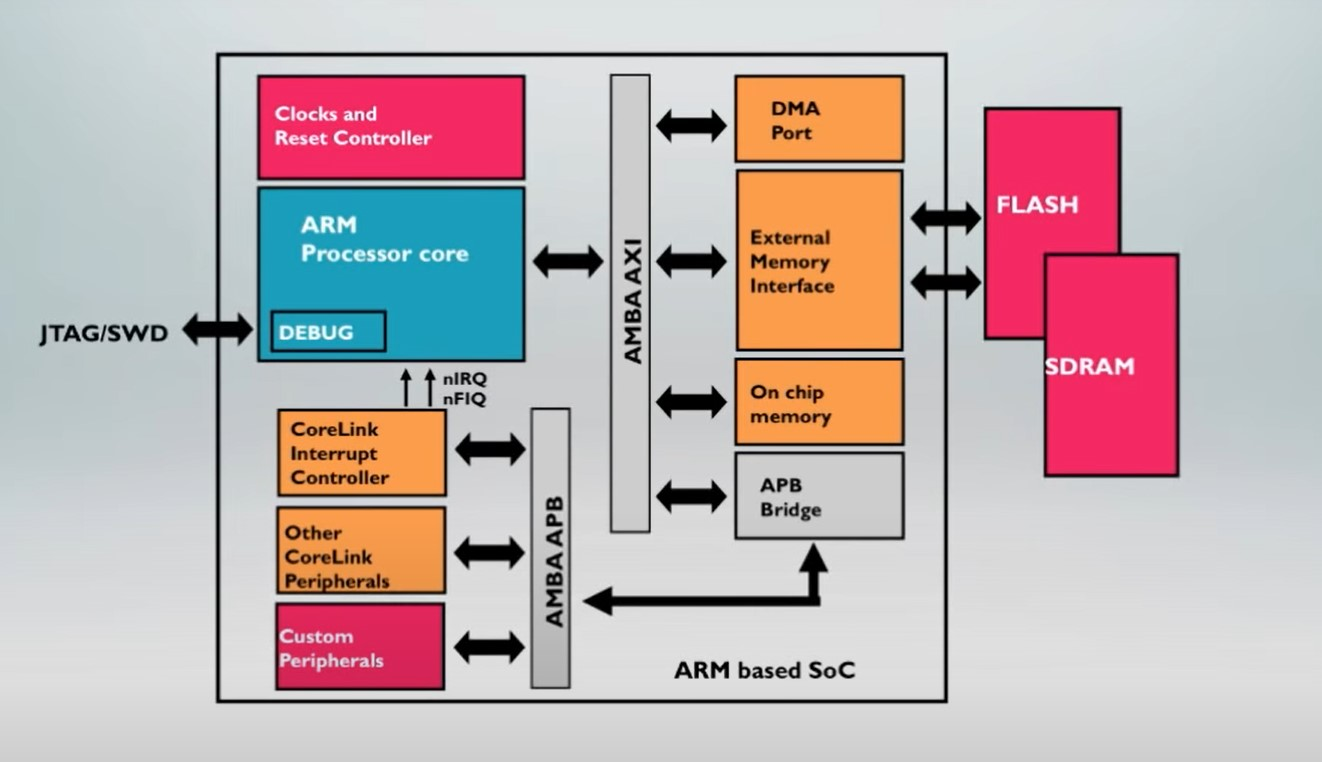
\includegraphics[width=\linewidth]{img/ARMCPUarchitecture.jpg}
    \caption{Een systematisch overzicht van een ARM processor \autocite{Shaw2013}}
\end{figure}

Het concept van een \textit{System-on-a-Chip} (SoC) beschrijft een complexe geïntegreerde schakeling, bestaande uit allerhande elektronische componenten zoals processorkernen, werkgeheugen, hardware logica, randapparatuur en andere elementen die onderling verbonden zijn door communicatiesystemen zoals interne databussen of netwerken \autocite{MathWorks2022}. Een SoC hoeft niet noodzakelijk gebruik te maken van ARM processoren, maar de meeste SoC’s die beschikbaar zijn op de markt doen dit wel. Een uitzondering op die regel is de Intel Atom x86 processorfamilie.

Een typische SoC maakt gebruik van een hele resem aan componenten, waarvan slechts enkele gebruikmaken van het intellectuele eigendom van ARM Ltd. De ARM processor die de dag van vandaag bestaat uit een meervoud aan kernen is diep ingebed in het toestel en is bijgevolg niet zichtbaar met het blote oog. De debug poort vormt de enige manier van directe toegang tot de processorkern(en) en wordt gebruikt bij het ontwerp, ontwikkeling, configuratie en debuggen van software. Er wordt algemeen aangenomen dat een debug-poort niet noodzakelijk is voor eindgebruikers. Daardoor wordt hij vaak verborgen of uitgeschakeld in eindproducten omdat deze poort vaak wordt misbruikt door hackers. De klok, zoals de naam al doet vermoeden, is verantwoordelijk voor het vastleggen van de kloksnelheid van een processor aan de hand van een constante stroom van impulsen \autocite{Shaw2013}. 

Alle componenten op een ARM SoC geïntegreerde schakeling zijn met elkaar verbonden door middel van een \textit{on chip interconnect bus}. Een bus is verantwoordelijk voor het transporteren van elektrische signalen door middel van een gemeenschappelijk transportmedium. De grote meerderheid van toestellen die gebruik maken van een ARM SoC doen dit via de ARM \textit{Advanced Microcontroller Bus Architecture} (AMBA) interface. Deze bestaat uit twee varianten die elk op hun beurt gespecialiseerd zijn in verschillende interacties. De AMBA AXI is de bus die zorgt voor interconnectie tussen onderdelen die een hoge doorvoersnelheid hebben zoals tussen de processor en het werkgeheugen. De AMBA APB is op zijn beurt verantwoordelijk voor het regelen van de gegevensstroom tussen de processor en randapparatuur. Dit gezegd zijnde, moet er opgemerkt worden dat de AMBA APB uitsluitend wordt gebruikt voor interne doeleinden. Verder hebben de meeste toestellen ook een zekere hoeveelheid werkgeheugen op de chip, evenals interfaces die leiden naar externe opslagmedia \autocite{Shaw2013}.

De hierboven vermelde componenten vormen slechts een introductie tot de elementen die men kan terugvinden op een \textit{System-on-a-Chip}. In de onderstaande figuur \ref{M1family} is er een gedetailleerde microscopische weergave terug te vinden van de processorarchitectuur van een \textit{Apple Silicon M1 processor}. Deze afbeelding laat de complexiteit van een moderne desktop ARM processor zien op een gestructureerde manier.

\begin{figure}[!htb]
    \centering
    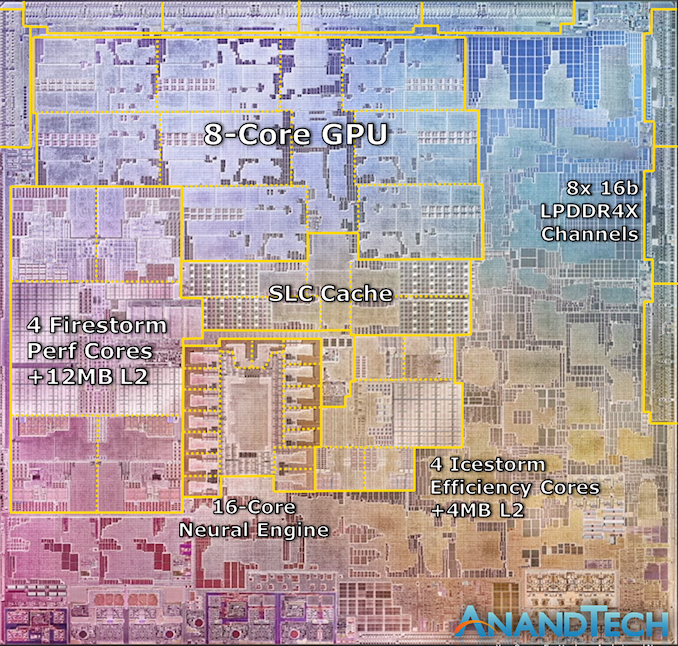
\includegraphics[width=\linewidth]{img/M1architecture.jpg}
    \caption{Een microscopische weergave van een M1 Apple Silicon processor \autocite{Frumusanu2020}}
    \label{M1family}
\end{figure}

\section{Verschillen tussen de ARM en x86 architectuur}
De processor van een elektronisch apparaat wordt vaak vergeleken met de hersenen. Deze analogie is echter slechts gedeeltelijk correct. Mensen en dieren hebben namelijk de mogelijkheid om zelfstandig en creatief na te denken zonder de behoefte aan externe instructies. Daartegenover staan processoren die nood hebben aan specifieke instructies alvorens ze een bepaalde taak, berekening of opdracht kunnen uitvoeren \autocite{Triggs2022a}. Het grootste aandeel van desktop- en laptopcomputers maken gebruik van x86 processors die zijn geproduceerd door Intel of \textit{Advanced Micro Devices} (AMD). Dit staat in schril contrast tegenover de wereld van de mobiele- en IoT apparaten die bijna universeel gebruik maken van ARM processoren \autocite{SarahHarris2015}.

Applicaties en programma’s worden ontworpen, ontwikkeld en gecompileerd met een bepaalde instructieset in gedachten. Tot op heden zijn dit voornamelijk de ARM en de x86 instructieset. Het is belangrijk om in gedachten te houden dat dit niet de enige gebruikte instructiesets zijn, maar procentueel gezien zijn deze dominant in hedendaagse elektronica. Zoals uitgelegd in het vorige hoofdstuk, is de ARM instructieset gebaseerd op de \textit{Reduced Instruction Set Computer} (RISC) instructieset. Deze staat tegenover de \textit{Complex Instruction Set Computing} (CISC) architectuur die wordt gebruikt voor x86 processors. Indien een chipfabrikant een processor wenst te ontwikkelen met een laag energieverbruik en een geringe warmteafgifte, dan is het van essentieel belang dat de gebruikte instructieset wordt ontworpen met eenvoud in gedachten. Dit is dan ook het geval bij de ARM instructieset die werd ontwikkeld met energieverbruik in gedachten. Daar tegenover staat de filosofie van de x86 processoren die worden ontworpen voor maximale performantie en interoperabiliteit \autocite{Triggs2022}.

Zoals eerder vermeld, is de x86 architectuur een voorbeeld van een CISC architectuur. Deze wordt gekenmerkt door instructies van een variabele lengte die vaak kleiner zijn dan 32 bits. Verder zijn er aanzienlijk meer instructies voorhanden op de CISC architectuur waarvan er vele in staat zijn om meerdere bewerkingen uit te voeren. Het nadeel van deze aanpak is dat complexe instructies vaak moeilijker te decoderen zijn en trager uitgevoerd worden. Dit staat tegenover de atomische RISC architectuur die gekenmerkt is voor zijn eenvoudige en relatief snelle instructies. Enkele voordelen van de CISC aanpak zijn: hogere performantie en instructies die meer werk leveren. Deze eigenschappen gaan echter wel gepaard met een hoger energieverbruik \autocite{SarahHarris2015}. 

De ARM architectuur heeft verder ook aanzienlijk meer registergeheugen. Een gevolg hiervan is dat er minder instructies nodig zijn om tussen registers te schakelen. ARM instructies werken tevens ook altijd in op het registergeheugen. Dit houdt in dat er expliciete laad- en opslaginstructies nodig zijn om gegevens tussen het werk- en registergeheugen te verplaatsen. X86 instructies daarentegen hebben de mogelijkheid om rechtstreeks in te werken op werk- en registergeheugen. Deze x86 eigenschap compenseert gedeeltelijk het gebrek van een laag aantal registers. Een ander verschil tussen beide architecturen is het feit dat ARM instructies drie operanden specificeren, namelijk één bestemming en twee bron operanden. Daartegenover staan de x86 instructies die slechts twee operanden specificeren, namelijk de bron en de bestemming. Dit houdt in dat x86 instructies altijd het bron operand moeten overschrijven met het resultaat, waardoor er niet meer terug naar de oorspronkelijke waarde kan worden gerefereerd \autocite{SarahHarris2015}. 

Tenslotte is ook de codering van instructiesets een pak complexer en minder gestroomlijnd op het x86 platform. De codering van instructies, een belangrijk aspect van een instructiesetarchitectuur, bepaalt hoe instructies en argumenten als binaire waarden worden gecodeerd in de machinecode van een systeem. De complexiteit en wanorde van x86 instructies is te verklaren aan het feit dat deze architectuur al enkele decennia wordt gebruikt in computerhardware. Dit houdt in dat er per processorgeneratie complexiteit werd toegevoegd bovenop de bestaande instructieset. Een voordeel van deze aanpak is zonder twijfel de uitstekende compatibiliteit van het platform, dit gaat echter ten koste van optimalisatie en specialisatie \autocite{SarahHarris2015}.

Verder is het ook belangrijk om op te merken dat zowel de ARM- als de x86 instructieset 64-bit processoren ondersteunen. Dit onder de vorm van de ARM AArch64 instructieset en de x86-64 instructieset \autocite{ARM2022a}. Moderne processoren zijn bijna allemaal 64-bit. Bij desktop-processoren is dit reeds het geval sinds de jaren negentig van de vorige eeuw. De transitie van 32-bit naar 64-bit gebeurde echter veel recenter voor mobiele toestellen. De Apple A7, die in 2012 werd uitgebracht, was de eerste 64-bit processor die werd gebruikt in een smartphone, dit zijnde de iPhone 5S. Alhoewel ARM processoren voornamelijk gebruikt worden in smartphones, is het gebruik ervan in desktops en laptops de laatste jaren explosief toegenomen. Dit is te wijten aan het succes van de \textit{Apple Silicon} toestellen, de populariteit van de \textit{single-board} computers zoals de Raspberry Pi en de opkomende trend van Windows on ARM laptops. Deze populariteit gaat gepaard met een uitdaging, namelijk het ondersteunen en maken van software die compatibel is met zowel de ARM alsook de x86 architectuur. Het compileren van \textit{native} software voor beide platformen is een uitstekende optie voor nieuwe programma’s en ontwikkelaars die bereid zijn om tijd te investeren in het hercompileren van hun reeds gecreëerde applicaties. Om het tekort aan software ondersteuning aan te kaarten, maken deze platformen gebruik van \textit{code emulation}. Dit proces omvat het vertalen van code die is gecompileerd voor de x86 architectuur naar code die compatibel is voor ARM processoren. Met deze aanpak komen er echter wel enkele problemen zoals lagere performantie en potentiële software instabiliteit. Dat gezegd zijnde is \textit{code emulation} een goede tussenoplossing die consumenten de mogelijkheid geeft om gebruik te maken van vertrouwde software \autocite{Triggs2022a}.

De ARM architectuur is het afgelopen decennium uitgegroeid tot de standaardkeuze als het gaat om smartphone processoren. Daar tegenover staat de x86 architectuur die al een dertigtal jaar de \textit{default} is op alle desktop platformen. Elke architectuur gaat gepaard met voor- en nadelen die het gevolg zijn van de eisen waarop ze werden ontworpen. De ARM en x86 architectuur zijn zeer verschillend op een technisch niveau, maar op het gebied van gebruiksdoeleinden voor consumenten bieden ze tegenwoordig een gelijkaardige ervaring. Experten stellen dat de x86 architectuur de komende jaren dominant zal blijven op desktop platformen, maar de unieke voordelen die voorkomen bij ARM processoren zorgen ervoor dat er na enkele decennia terug meer competitie is op de markt \autocite{Triggs2022}.

\section{Prestatie per watt van ARM processoren}
\subsection{Hoe de wet van Moore evolueerde naar die van Koomey}
De evolutie van processors in de vorige eeuw werd gekenmerkt door razendsnelle innovatie en baanbrekende ideeën die vaak gepaard gingen met succes. Gordon Moore, een van de medeoprichters van de technologiegigant Intel, merkte al snel een opvallende trend op in die evolutie, namelijk een verdubbeling van het aantal transistoren in een processor iedere 24 maanden. Een transistor is een sturend element in een elektrische schakeling en tevens de bouwsteen van computers en geïntegreerde elektrische schakelingen. Dit inzicht kreeg de naam “Moore’s law” en werd gebruikt als de maatstaf waarmee het huidige tempo van innovatie en vooruitgang mee werd afgemeten. Deze werd het laatste decennium vaak beschouwd als een zelfvervullende voorspelling omdat fabrikanten van processoren de wet van Moore vaak gebruikten als een soort van doelstelling die behaald moest worden \autocite{Schaller1997}.

\begin{figure}[!htb]
    \centering
    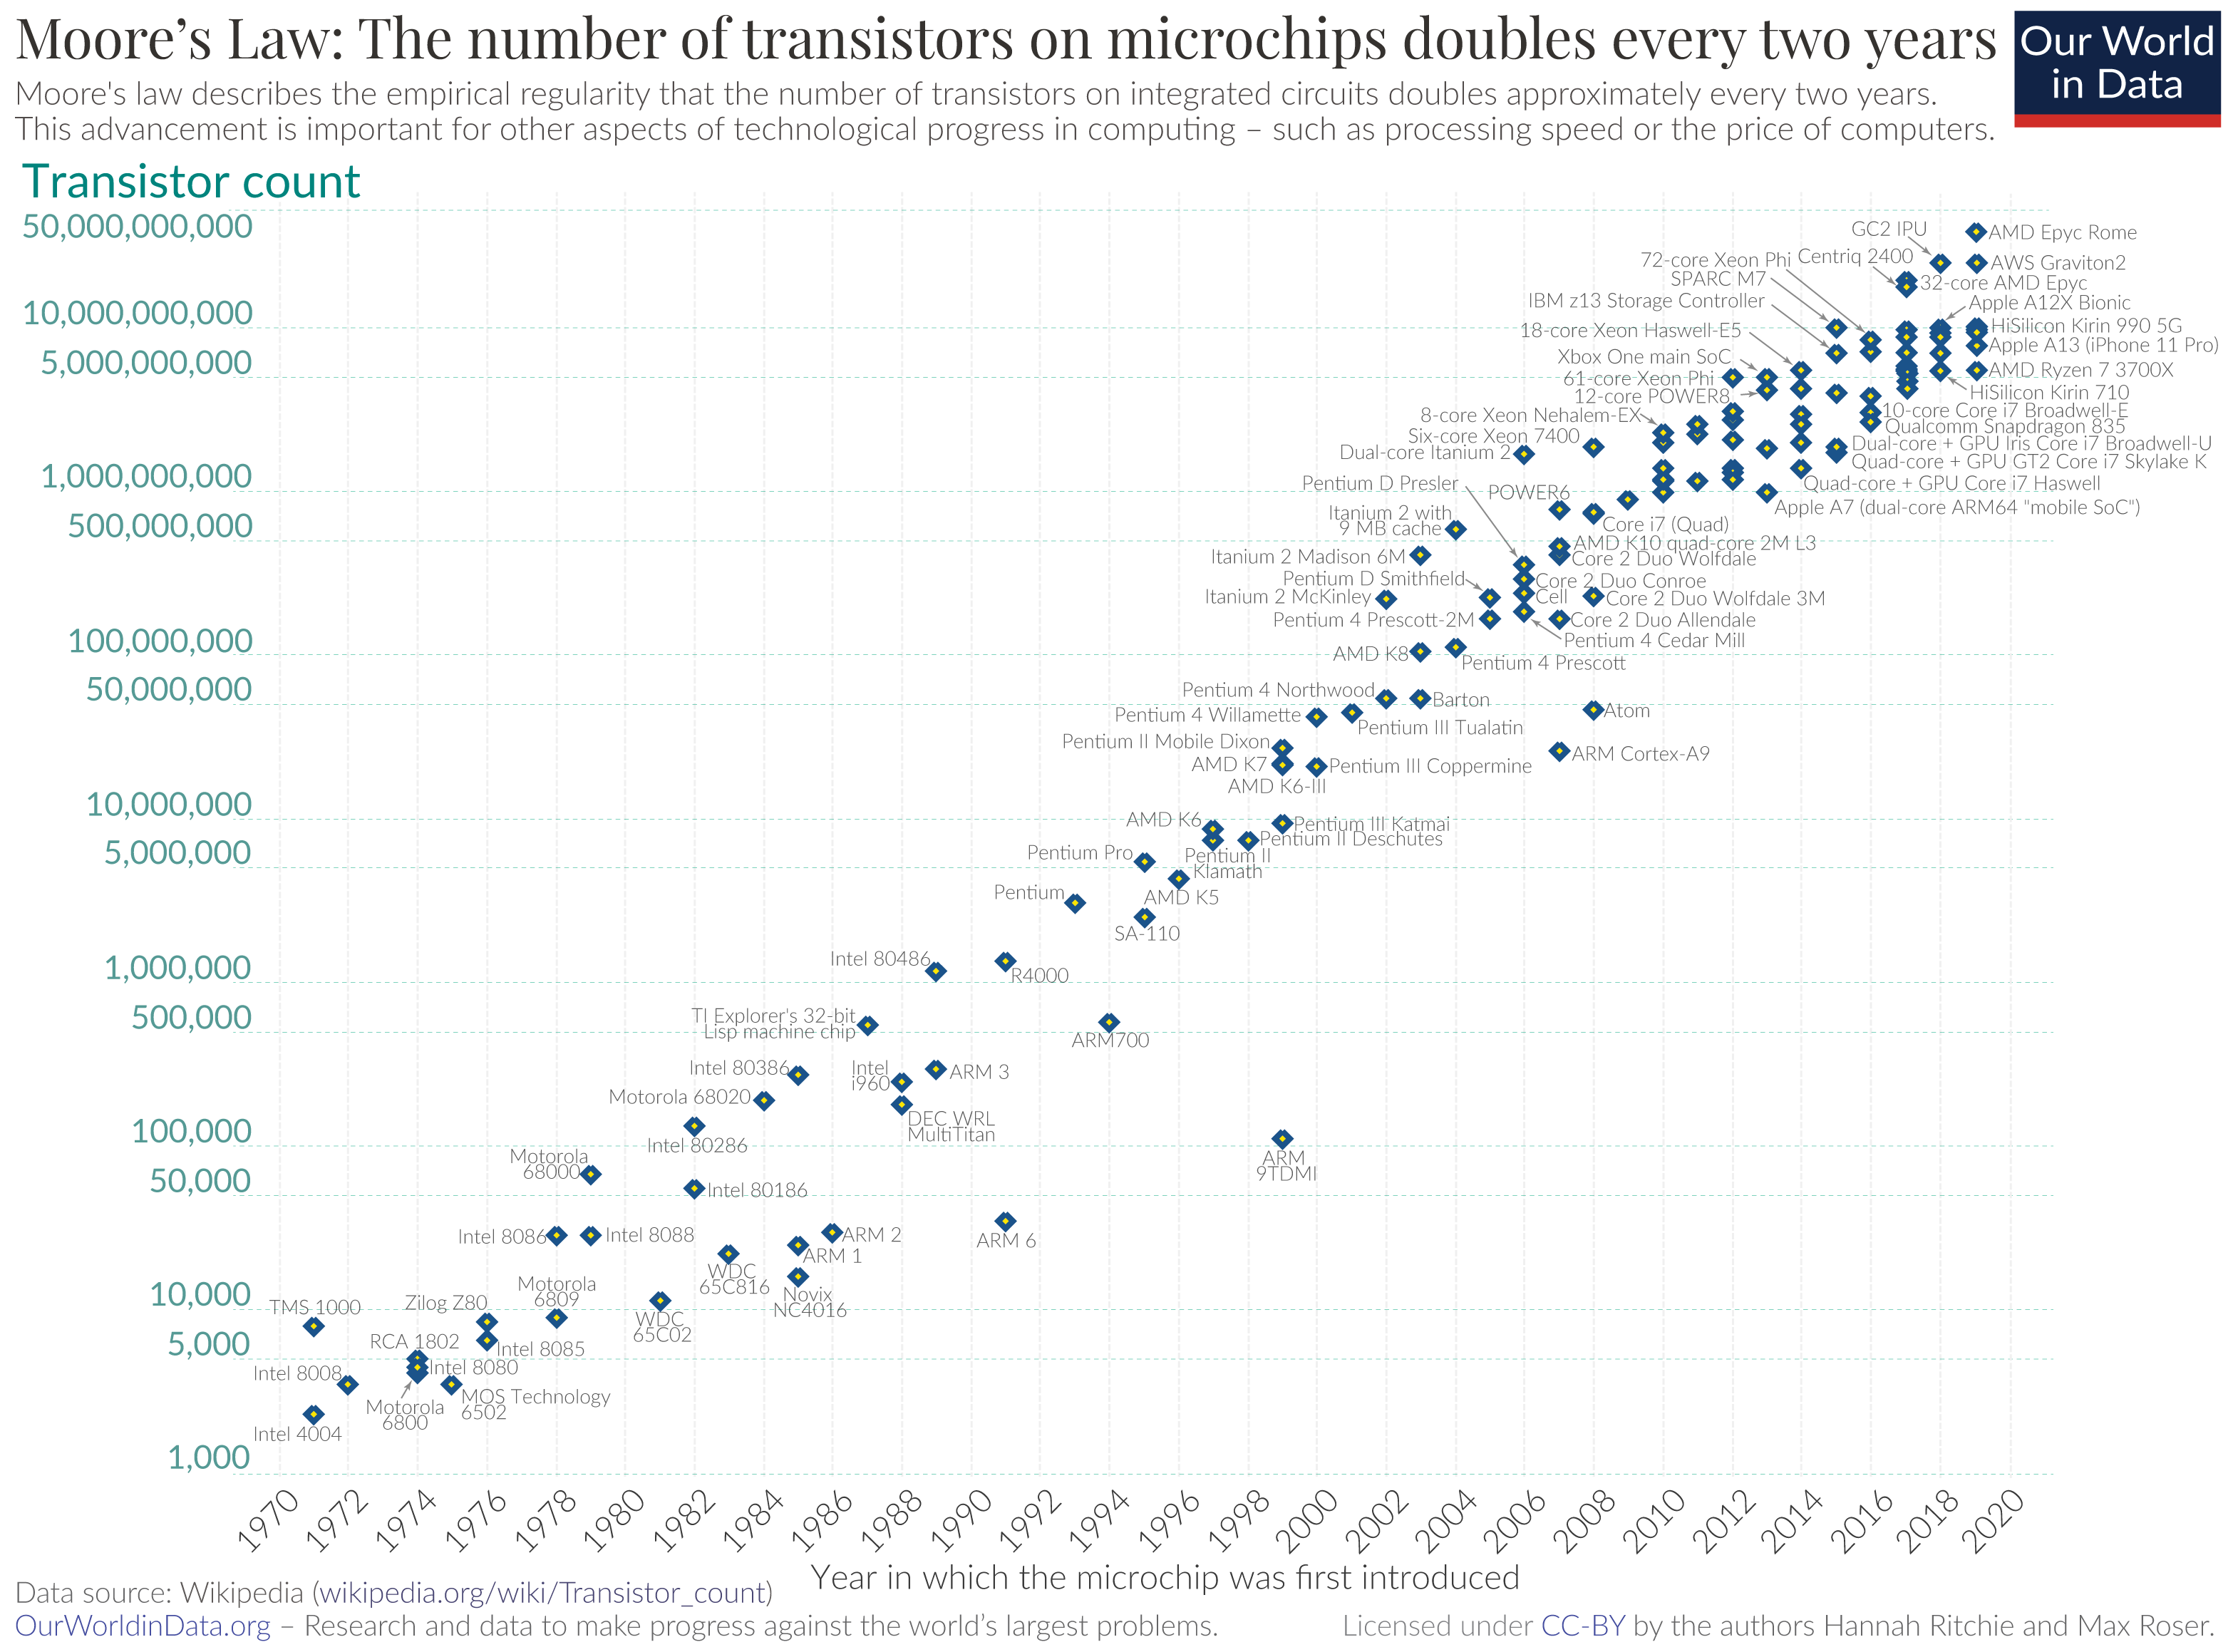
\includegraphics[width=\linewidth]{img/transistorcountovertime.jpg}
    \caption{Een grafische voorstelling van het aantal transistoren in processoren \autocite{HannahRitchie2020}}
\end{figure}

Als de specificaties van een bepaalde processor worden bestudeerd, dan valt het op dat fabrikanten spreken over de lithografie die wordt uitgedrukt in nanometer. Het getal dat gekoppeld wordt aan de lithografie staat gelijk aan de grootte van de transistoren die gebruikt worden. Kleinere transistors leidden tot een lager stroomverbruik van de processor \autocite{Heddings2019}.

De periode tussen 2015 en 2021 wordt gekenmerkt door een gebrek aan vooruitgang op het gebied van lithografie, dit is voornamelijk het geval bij Intel, de grootste chipfabrikant ter wereld. In deze periode maakten alle generaties van Intel processoren namelijk gebruik van de 14 nanometer lithografie. Dit is echter niet toevallig aangezien het ontwikkelen van nog kleinere transistoren gepaard gaat met kwantummechanische problemen \autocite{Intel2021}.

\begin{figure}[!htb]
    \centering
    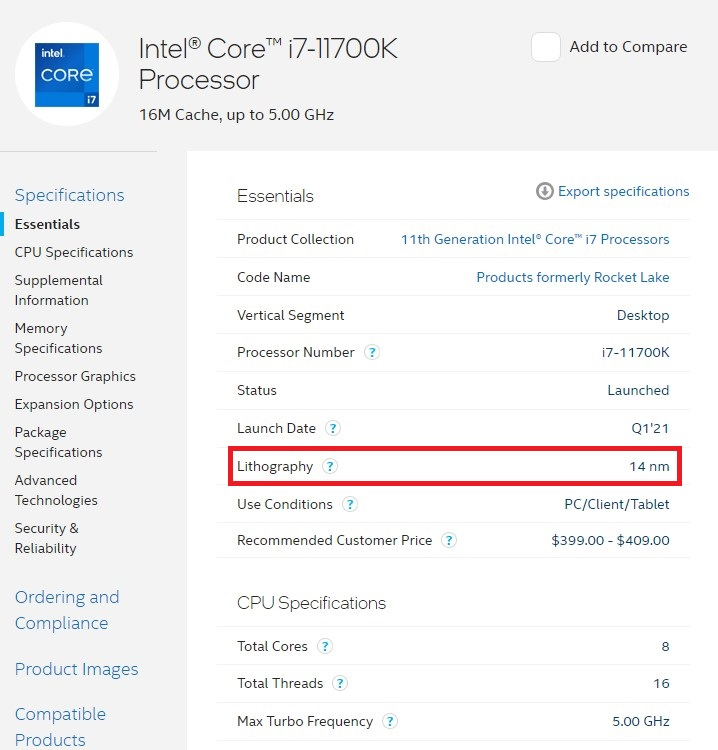
\includegraphics[width=\linewidth]{img/11700k.jpg}
    \caption{Specificaties van de Intel 11700K \autocite{Intel2021}}
\end{figure}

Om dit gebrek aan innovatie te verlichten, spitsen chipfabrikanten zich toe op andere 
factoren en innovaties die bijdragen tot betere performantie. Een van deze nieuwe technologieën is \textit{3d stacking}. Zoals de naam doet vermoeden is dit een driedimensionale geïntegreerde schakeling die wordt bekomen door het stapelen van processor onderdelen \autocite{DeBenedictis2017}. De performantie mogelijkheden die komen bij het gebruik van \textit{3d stacking} worden ook beaamd door \textcite{Aitken2019}. Een voorbeeld van een processor die ontworpen is met deze nieuwe technologie is de AMD Ryzen 7 5800X3D. Deze maakt gebruik van verticaal gestapeld \textit{cache} geheugen, wat ertoe leidt dat deze processor toegang heeft tot een aanzienlijke hoeveelheid \textit{cache} geheugen. Een voordeel van deze aanpak is dat data minder vaak moet worden uitgewisseld tussen cache- en werkgeheugen \autocite{AMD2022}.

Aangezien “Moore’s law” de komende jaren minder relevant zal worden omwille van de inherente kwantummechanische eigenschappen die komen bij het verkleinen van de processor lithografie, is de industrie aan het uitkijken naar een nieuwe relevante maatstaf. Velen geloven dat deze komt in de vorm van prestatie per watt. In de wereld van de informatica en computerwetenschappen is prestatie per watt een indicator voor het energierendement van een bepaalde computerarchitectuur of computerhardware. De term prestatie per watt kan vrij letterlijk genomen worden, het berekent namelijk de verwerkingscapaciteit die een processor/computer kan leveren per verbruikte watt aan energie \autocite{Audiopedia2017}.

Energieverbruik, duurzaamheid en de ecologische voetafdruk zijn concepten waar elke soort industrie mee wordt geconfronteerd. Dit gezegd zijnde is de ecologische voetafdruk en het energieverbruik van de hoogtechnologische industrie lang onder de radar gebleven. Nochtans is deze sector verantwoordelijk voor veel meer energieverbruik dan men aanvankelijk zou inschatten. De servers die gepaard gaan met het \textit{client-server} model verbruiken namelijk een aanzienlijke hoeveelheid energie. Dit omwille van de energie hongerige processoren en de aanzienlijke koelinstallaties die nodig zijn om de apparatuur in datacenters af te koelen. Verder moet er ook rekening gehouden worden met de huidige digitale kloof die zich afspeelt tussen eerste- en derde wereldlanden. Er wordt voorspeld dat deze kloof de komende jaren aanzienlijk zal krimpen. Dit houdt in dat er binnenkort 3,7 miljard mensen zijn die nood zullen hebben aan hoogtechnologische toestellen en de bijbehorende datacenters. Met deze kennis in het achterhoofd roepen deskundigen op tot een mentaliteitsverandering \autocite{Aitken2021}.


De mentaliteit die hoort bij de wet van Moore roept indirect op tot het ontwikkelen van processoren die keer op keer meer performantie bieden ongeacht het energieverbruik, het spreekt voor zich dat deze denkwijze achterhaald is. De industrie moet ernaar streven om processoren te ontwikkelen met een focus op prestaties per watt. Deze denkwijze sluit aan bij het “Koomey’s law” model. Deze wet die bedacht is door Jonathan Koomey, een Stanford University professor, stelt dat de energie-efficiëntie van computers ongeveer elke 18 maanden verdubbelt, in tegenstelling tot de wet van Moore, die stelt dat de verwerkingskracht elke 18 tot 24 maanden verdubbelt \autocite{Koomey2011}.

\subsection{Introductie tot benchmarking}
In de volgende secties zal er gesproken worden over de performantie van moderne ARM processoren. Om de capaciteiten van ARM en x86 processoren te vergelijken wordt er gebruik gemaakt van \textit{benchmark} software. Dit zijn gestandaardiseerde prestatiemetingen die de capaciteit van computerhardware evalueren en vergelijken. Cinebench R23 is een \textit{benchmark} softwarepakket die compatibel is met alle moderne hardware platformen zijnde x86 en ARM. Het doel van de test is om een bepaalde scène te renderen die maximaal gebruik maakt van de rekenkracht van een processor. Om het huidige tempo van hardware-evolutie bij te houden wordt het Cinebench softwarepakket voortdurend bijgewerkt. De Cinebench \textit{benchmark} kan uitgevoerd worden in twee modi, namelijk de \textit{single-threaded} modus die maar één processorkern benut en de \textit{multi-threaded} modus die gebruik maakt van alle processorkernen \autocite{Maxon2022}. Aangezien het gros van de hedendaagse software geoptimaliseerd is voor multikernprocessors, zullen de onderliggende secties zich voornamelijk toespitsen op de resultaten van de \textit{multi-threaded} modus in Cinebench R23. De \textit{single-threaded} score dient echter niet genegeerd te worden aangezien deze voornamelijk representatief is bij alledaags gebruik.

\subsection{Apple Silicon}
\subsubsection{M1}
Sinds november 2020 maakt Apple gebruik van ARM processoren in hun Mac aanbod. De eerste desktop ARM chip die Apple heeft ontworpen is de M1, deze is gericht op het “goedkopere” segment van hun desktops en laptops dat tevens een focus heeft op mobiliteit. Deze toestellen zijn gericht op consumenten en studenten die niet noodzakelijk een nood hebben aan hoge prestaties. Dat gezegd zijnde is deze chip zeer indrukwekkend voor een eerste poging tot desktop ARM processoren. De M1 is uitgerust met acht processorkernen en verbruikt bij alledaags gebruik 7 watt. Bij maximale prestaties is de M1 in staat om 20 watt te verbruiken. Als men kijkt naar onderstaande figuur Cinebench R23 M1 dan is het duidelijk dat de M1 processor indrukwekkende prestaties levert. Een \textit{multi-threaded} score die 7833 bedraagt is op zich al behoorlijk indrukwekkend, maar zeker wanneer men deze in context plaatst met de vorige generatie aan Apple toestellen die u onderaan de grafiek kunt vinden. Het is voornamelijk de \textit{single-threaded} score die indrukwekkend is bij de M1. Deze is namelijk quasi gelijk aan de score van de AMD Ryzen 5950X. Dit is een processor die 105 watt verbruikt en die enkel te verkrijgen is in hoogwaardige desktops \autocite{Frumusanu2020a}.

\subsubsection{M1 Pro}
\raggedbottom
De M1 Pro \textit{Apple Silicon} chip is voornamelijk ontwikkeld voor ICT'ers en professionals op het gebied van foto- en videografie. Het spreekt dus voor zich dat deze processor is ontworpen met performantie in gedachten. Dit kan ook beaamd worden door het toonaangevende resultaat in de Cinebench R23 \textit{multi-threaded} test. Dit resultaat wordt des te meer indrukwekkend wanneer men in gedachten houdt dat de M1 Pro 30 watt aan energie verbruikt bij maximale prestaties tegenover zijn naaste concurrent de Ryzen 9 5900HX die 45 watt verbruikt \autocite{Schiesser2021}.

\subsection{Snapdragon 8cx}
\raggedbottom
De Snapdragon 8cx reeks van processoren is ontwikkeld door Qualcomm en is uitsluitend gericht op de markt van de Windows on ARM toestellen. Deze worden vrijwel allemaal gekenmerkt door een dun profiel, een focus op mobiliteit en indien mogelijk, passieve koeling. Dit houdt in dat de processor niet wordt gekoeld door een ventilator maar door een koelplaat die in staat is om warmte passief af te geven. Deze manier van koeling is enkel mogelijk bij processoren die een geringe hoeveel warmte uitstoten. De Snapdragon 8cx2 die beschikbaar is sinds 2020 verbruikt slechts 7 watt, desondanks deze uitstekende efficiëntie is hij toch in staat om te concurreren met sommige energiezuinige varianten van de Intel Core i5 \autocite{Qualcomm2020}. Deze geclaimde performantie dient echter gekaderd te worden. Wanneer de performantie van de 8cx en de gelijkaardige SQ2 worden vergeleken met deze van de \textit{Apple Silicon} M1 dan valt er op dat de Qualcomm chips niet in staat zijn om te concurreren. Sterker nog, de hierboven vermelde M1 chip levert zelfs betere performantie dan de Snapdragon chip onder gevirtualiseerde omstandigheden. Virtualisatie software heeft nochtans een aanzienlijke impact op performantie. Dit toont aan dat Qualcomm nog een heleboel werk heeft vooraleer het effectief in staat is om te concurreren met Apple, Intel en AMD \autocite{Wankhede2020}.

\begin{figure}[!htb]
	\centering
	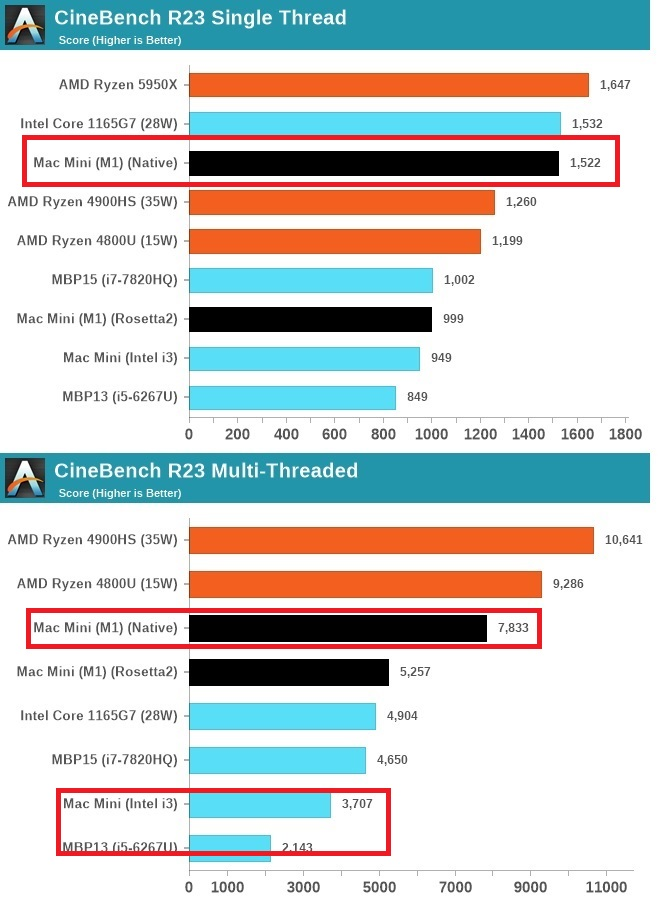
\includegraphics[width=\linewidth]{img/m1cinebenchr23.jpg}
	\caption{Cinebench R23 M1 \autocite{Frumusanu2020a}}
\end{figure}
\begin{figure}[!htb]
	\centering
	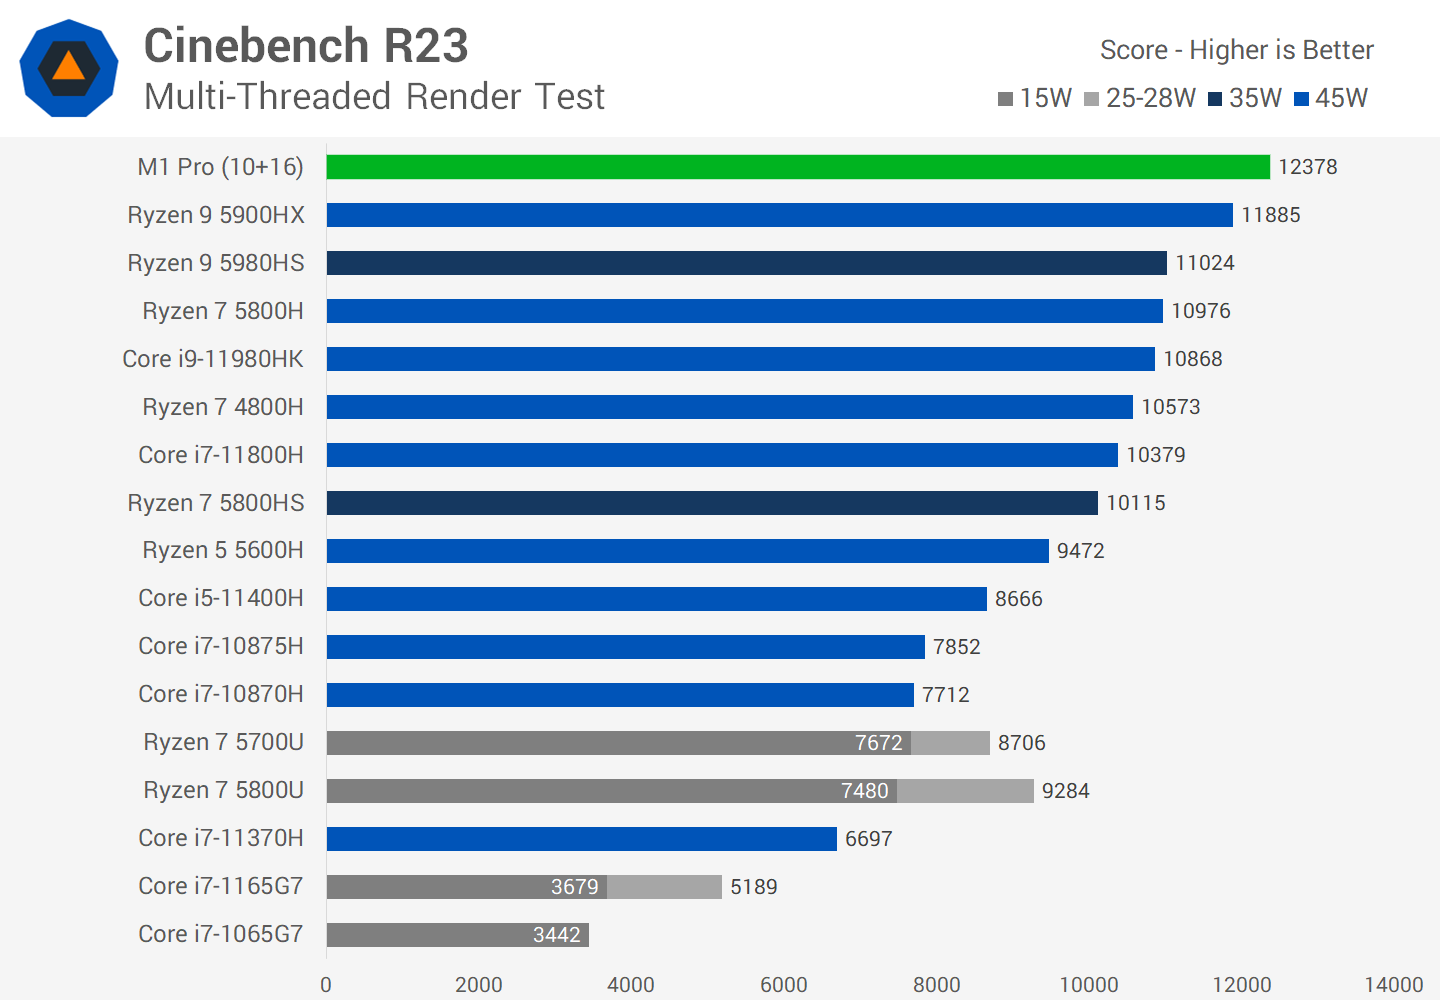
\includegraphics[width=\linewidth]{img/m1procinebenchr23.jpg}
	\caption{Cinebench R23 M1 Pro \autocite{Schiesser2021}}
\end{figure}

\subsection{Amazon graviton}
\subsubsection{De ecologische impact van datacenters}
Datacenters zijn noodzakelijk bij het gebruik van het \textit{client-server} model. Wat velen niet weten is dat deze datacenters verantwoordelijk zijn voor 3\% van het wereldwijde elektriciteitsverbruik. Dit houdt in dat datacenters meer elektriciteit verbruiken dan het Verenigd Koninkrijk, ze zijn tevens ook verantwoordelijk voor 2\% van de wereldwijde uitstoot van broeikasgassen. Tot overmaat van ramp wordt deze dure computerhardware op het einde van zijn levenscyclus vaak gedumpt als \textit{e-waste} terwijl deze hergebruikt kan worden voor andere doeleinden. \textit{E-waste} vertegenwoordigt in totaal 2\% van het wereldwijde vaste afval en 70\% van het giftige afval \autocite{Supermicro2018}.

Het is echter niet de processor of de grafische kaart die verantwoordelijk is voor het torenhoge energieverbruik van een server, de sluipmoordenaar is de koelingsapparatuur die nodig is voor het afkoelen van de computerhardware. De gemiddelde temperatuur van datacenters bedraagt tussen de 21 en 24 graden Celsius. Deze relatief frisse omgeving is nodig om de levensduur van de hardware maximaal te houden en om 99.999\% betrouwbaarheid te garanderen. Waterkoeling, luchtkoeling en airconditioning zijn de meest gebruikte methodes om de temperatuur van een datacenter optimaal te houden \autocite{Miller2022}.

Een manier waarop datacenters hun warmte uitstoot en energieverbruik kunnen minimaliseren is het regelmatig bijwerken van de hardware in hun serverapparatuur. Deze upgrades kunnen datacenters helpen besparen op hun energiefactuur alsook het minimaliseren van hun ecologische voetafdruk. Het spreekt voor zich dat nieuwe processoren en apparatuur een boost zullen leveren op het gebied van performantie en energiezuinigheid. Bij deze upgrades moet een datacenter wel een concrete strategie plannen met betrekking tot de verouderde hardware \autocite{Supermicro2018}. Een correcte strategie is het hergebruiken en herverpakken van computerhardware zoals processoren, grafische kaarten, moederborden en werkgeheugen in een nieuw product aangezien deze onderdelen een levensduur hebben die aanzienlijk hoger is dan de gemiddelde gebruiksduur. Onderdelen zoals opslag die komt in de vorm van \textit{solid state drives} of harde schijven kunnen niet hergebruikt worden omwille van confidentialiteit. Het hergebruiken van computerhardware die afkomstig is uit server toestellen past in het concept van \textit{upcycling}, de circulaire economie en de ladder van Lansink \autocite{VanAcker2017}.

\subsubsection{De AWS Graviton Processor}
Amazon staat bekend door zijn online webwinkel, dit is echter slechts één item in hun portfolio van online webservices. Amazon Web Services (AWS) is een \textit{cloudcomputing} dienst die het mogelijk maakt voor particulieren en bedrijven om een bepaalde serverconfiguratie te huren voor een bepaalde of onbepaalde termijn. Enkele technologiereuzen die gebruik maken van het AWS platform zijn onder andere Netflix, Discovery Channel, Formula 1 en Epic Games \autocite{Amazon2022}. Op heden is het AWS cloudplatform de marktleider met als naaste concurrenten Microsoft Azure en het Google Cloud Platform \autocite{Alexandre2021}.

De AWS Graviton processoren steunen op de Arm Neoverse N1 en zijn ontworpen door AWS en ARM. Deze worden gebruikt voor het hosten van de \textit{Amazon Elastic Compute Cloud 2} (EC2). Een voordeel die komt bij het ontwikkelen van processoren voor eigen gebruik is dat het mogelijk is om rekening te houden met de beoogde toepassingen. In het geval van de Graviton processoren zijn dit rekenkundige toepassingen, automatisatie, compressie, machinaal leren en \textit{floating point} performantie \autocite{arm2021}. Amazon claimt dat de AWS Graviton processoren een prijs-prestatieverhouding kunnen leveren die 40\% beter is dan vergelijkbare x86-gebaseerde instanties, dit terwijl het energieverbruik 60\% lager ligt \autocite{Amazon2021}.

\subsection{Raspberry Pi 4}
De eerste generatie van de Raspberry Pi werd geïntroduceerd in 2012 en deze was meteen een succes bij hobbyisten en technologiefanaten. De nieuwste variant, de Pi 4 is sinds 2020 beschikbaar voor het grote publiek en deze bouwt voort op het nalatenschap van de vorige generaties. De Pi 4 verbruikt 3,4 watt aan energie bij alledaags gebruik en 7,6 watt onder zware belasting. Dit cijfer ligt 17\% hoger dan de vorige variant, de Pi 3B+, maar het is belangrijk om te kaderen dat dit energieverbruik nog steeds aanzienlijk lager is dan andere computers. Een van de redenen voor dit “hogere” stroomverbruik is de ARM Cortex-A72 die ervoor zorgt dat de Pi 4, de eerste Raspberry Pi is die kan beschouwd worden als een desktop vervanger. De performantie van de vorige modellen was goed genoeg voor recreationeel gebruik, maar zodra de processor werd belast met alledaagse taken, kwam deze tekort. Daartegenover staat de Raspberry Pi 4 die de mogelijkheid heeft om videosignalen uit te voeren naar twee 4K schermen. Deze beschikt tevens over een Ethernet poort die Gigabit snelheden (125 MBps) kan ondersteunen. In de Apache Web Serving \textit{benchmark} scoorde de Pi 4 40\% hoger dan zijn voorganger en maar liefst meer dan het dubbele dan de Pi 3B+ in de PHPBench test \autocite{Piltch2020}.

De filosofie van de Raspberry Pi toont aan dat performantie maar één van de vele metrieken is die bijdraagt tot een goede gebruikerservaring. Een categorie van toestellen die aantoont dat performantie niet allesomvattend is, zijn de Internet of Things (IoT) apparaten. Deze categorie maakt namelijk vaak gebruik van processoren of technologieën die reeds tien jaar bestaan en dit zonder merkbaar prestatieverlies \autocite{Aitken2019}. 

\section{Marktonderzoek: het aanbod van ARM computers in 2022}
In de vorige hoofdstukken werd de architectuur van ARM processoren onderzocht alsook de voor- en nadelen die gepaard gaan bij het gebruik van deze architectuur. Deze sectie doet dienst als een marktonderzoek waarin wordt onderzocht welke laptop en desktop computers er beschikbaar zijn met ARM processoren. De categorie van de \textit{single-board} computers zal ook bestudeerd worden aangezien deze de laatste jaren spectaculair is toegenomen in populariteit omwille van hobbyisten en talrijke industriële toepassingen.

\subsection{Windows on ARM}
Microsoft speelt al sinds 2012 met het idee om energiezuinige ARM processoren te gebruiken in laptop-tablet hybride toestellen. Het besturingssysteem dat toen werd ontwikkeld was Windows RT. Deze eerste generatie van Windows ARM toestellen werd niet goed ontvangen door consumenten omwille van de geringe hoeveelheid aan programma's die beschikbaar waren op het 32-bit platform. Omwille van die desinteresse van software ontwikkelaars en consumenten stierf het platform een stille dood in 2016. Alhoewel Windows RT en de bijbehorende Microsoft Surface RT de geschiedenis zijn ingegaan als een commerciële flop, leerde het Microsoft en de software \textit{community} een belangrijke les. Gebruiksvriendelijkheid en de beschikbaarheid van de meest gebruikte software is vitaal voor de levensvatbaarheid van een besturingssysteem \autocite{Triggs2022}. 

Het Windows 10 on ARM desktop besturingssysteem, dat kan beschouwd worden als de opvolger van Windows RT, maakte zijn introductie in 2017. Met die introductie kwam een samenwerkingsverband tot stand tussen Microsoft en Qualcomm. Qualcomm is gekend voor het ontwikkelen van de bekende Snapdragon ARM processoren die gebruikt worden in Android smartphones en tablets. Elke partner is verantwoordelijk voor het naar voren brengen van een concurrentievoordeel. Het doel van Microsoft is om een 64-bit desktop besturingssysteem te ontwikkelen die innovatief doch herkenbaar is voor consumenten. Zoals eerder besproken, is software ondersteuning op een desktop platform even essentieel als de technologie die achter het platform steekt. Qualcomm is verantwoordelijk voor het ontwikkelen van de 8cx SoC’s die uitsluitend gericht zijn op het laptop segment van de markt. De introductie van Windows 11 on ARM maakt het mogelijk voor gebruikers om x86 software te emuleren. Dit houdt in dat bestaande x86 programma’s uitvoerbaar zijn op dit nieuwe platform. Deze aanpak gaat echter wel gepaard met een aantal problemen in de vorm van een geringe hoeveelheid prestatieverlies en een aantal stabiliteitsproblemen \autocite{Carrasqueira2022}.

\begin{figure}[!htb]
    \centering
    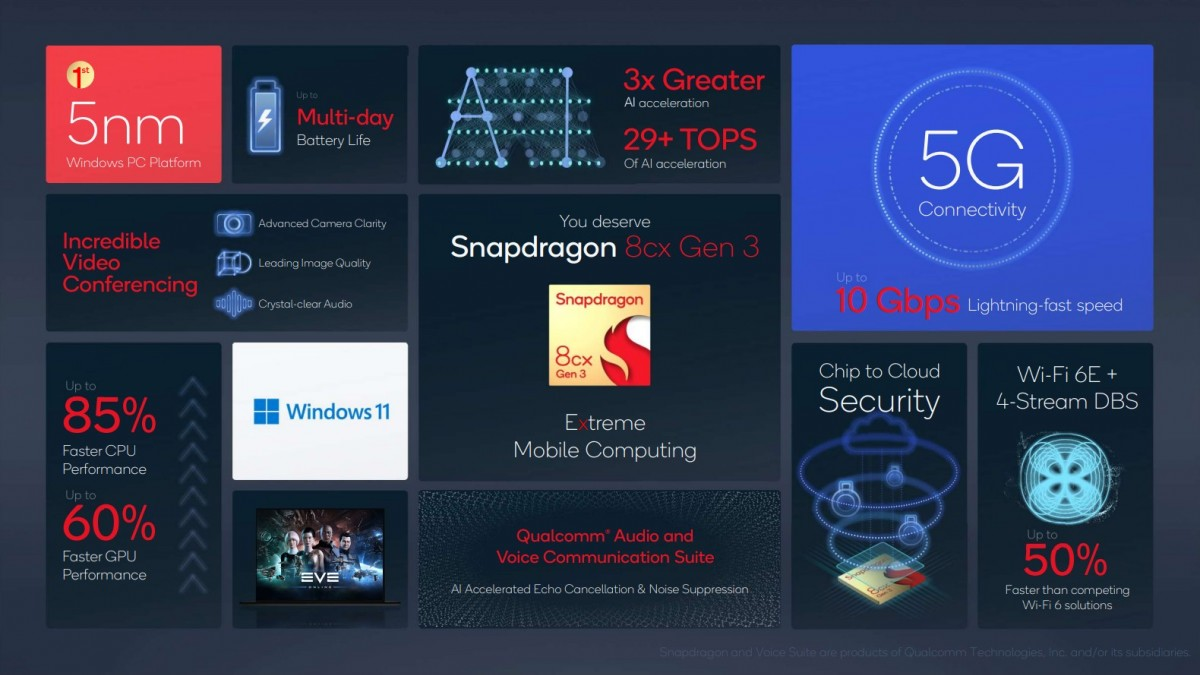
\includegraphics[width=\linewidth]{img/gsmarena_001.jpg}
    \caption{Een overzicht van de Snapdragon 8cx Gen 3 processor \autocite{Peter2021}}
\end{figure}

Laptops die berusten op het Windows on ARM besturingssysteem delen enkele belangrijke kenmerken zoals mobiliteit, toonaangevende batterijduur en connectiviteit. Door het gebruik van Snapdragon processoren hebben vele Windows on ARM laptops de mogelijkheid om verbinding te maken met mobiele 4G(LTE) of 5G netwerken. Deze eigenschap zorgt ervoor dat professionals die vaak moeten reizen of werken buiten de klassieke kantooromgeving, geïnteresseerd zijn in dit type toestellen. Samsung, Microsoft, Lenovo en Acer zijn de belangrijkste producenten van laptops die gebruikmaken van Snapdragon 8cx-processoren \autocite{Matte2022}.

\subsection{Apple Silicon}
Gedurende het jaarlijkse \textit{World Wide Developer Congress} (WWDC) dat plaatsvond op 22 juni 2020, kondigde Apple Inc. aan dat de Mac productlijn van desktops en laptops zou beginnen aan een twee jaar durende transitie van Intel x86 processoren naar ARM processoren. Deze reeks van SoC’s kreeg later de naam \textit{Apple Silicon}. De gevolgen van deze transitie zijn niet de minste. Elk toestel dat Apple ontwerpt, gaande van de iPhone tot de Mac zal voortaan gebruikmaken van een processor die door het bedrijf zelf is ontworpen. De belangrijkste voordelen die een resultaat zijn van deze overgang zijn ongetwijfeld energie-efficiëntie, performantie en software compatibiliteit in het volledige gamma van toestellen \autocite{Liao2022}.

Om ervoor te zorgen dat ontwikkelaars en software bedrijven klaar zijn voor deze overgang, heeft Apple een \textit{developer transition kit} ontwikkeld. Dit is als het ware een desktop Mac die gebruik maakt van een A12Z Bionic SoC die ontworpen is voor de iPad. Deze transitie kit belicht een van de grootste nadelen die komt bij de transitie van Intel x86 processoren naar \textit{Apple Silicon}, zijnde dat software specifiek moet ontworpen worden voor dit nieuwe platform. Voor ontwikkelaars van applicaties die reeds op de markt zijn volstaat het om hun applicatie opnieuw te compileren op een apparaat die voorzien is van een \textit{Apple Silicon} processor. Andere programma's zullen gebruik moeten maken van de \textit{Rosetta 2 translation layer}. Deze naam is gekozen naar analogie met de steen van Rosetta die dienst deed voor het vertalen van het hiërogliefenschrift. Een nadeel bij het gebruik van deze translation layer is dat software wordt uitgevoerd door het gebruik van virtualisatie. Dit houdt in dat de performantie van een applicatie die gebruik maakt van de \textit{Rosetta 2 translation layer}, lager zal zijn dan deze van een applicatie die ontworpen is voor de \textit{Apple Silicon} architectuur \autocite{Apple2020}.

Op 8 maart 2022 werd de Mac Studio bekend gemaakt aan het grote publiek. De release van deze desktop Mac computer betekent het einde van de overgangsperiode van Intel x86 naar \textit{Apple Silicon}. De eerste generatie van \textit{Apple Silicon} processoren bestaat uit de M1, M1 Pro, M1 Max en de M1 Ultra. De snelheid waarmee deze nieuwe generatie aan processoren is ontworpen is te danken aan de schaalbaarheid van de ARM architectuur. Vanaf dit moment zullen alleen nog maar toestellen met \textit{Apple Silicon} ARM processoren uitgebracht en geproduceerd worden, waarmee de periode van ARM dominantie op het Mac desktop platform definitief is ingeluid \autocite{Apple2022}. 

\begin{figure}[!htb]
    \centering
    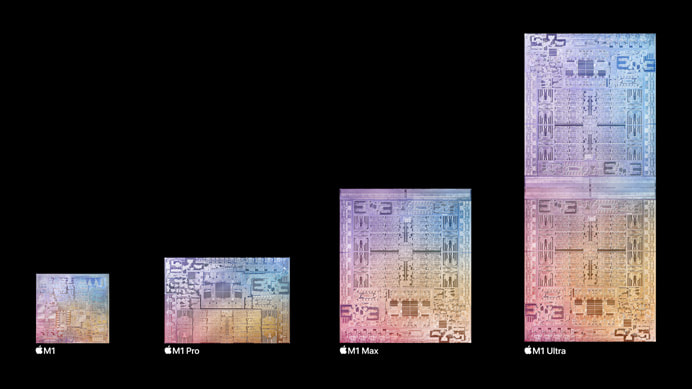
\includegraphics[width=\linewidth]{img/Apple-M1-chip-family-lineup.jpg}
    \caption{Een overzicht van de eerste generatie Apple Silicon processors \autocite{Apple2022}}
\end{figure}

\subsection{Single-board computers}
Een \textit{single-board computer} kan gedefinieerd worden als een printplaat die alle componenten bevat die nodig zijn voor een werkende computer. Dit zijn de centrale verwerkingseenheid (cve), werkgeheugen, opslag, input/output (I/O) en verbindingsmogelijkheden zoals Ethernet \autocite{Pcmag2022}. Deze toestellen staan bekend voor hun kleine oppervlakte en kostprijs. Dit verklaart de populariteit van het gebruik van deze toestellen in de onderwijsmarkt en bij private hobbyprojecten. Een andere markt waar deze toestellen in populariteit winnen is deze van de industriële toepassingen.

\subsubsection{Raspberry Pi}
De reden achter de creatie van de Raspberry Pi is eenvoudig doch fascinerend. Deze categorie van \textit{single-board} computers werd ontwikkeld om kinderen en jongeren te inspireren om te kiezen voor een carrière in de computerwetenschappen of om ze in ieder geval te interesseren in de werking van computers en software \autocite{Severance2013}. Dit verklaart het simpele bouwproces, de lage kost en de robuustheid van deze toestellen die vaak voor minder dan 100 euro verkrijgbaar zijn. 

De meest recente toevoegingen aan de familie van Raspberry Pi \textit{single-board} computers zijn de Pi 4 die wordt geleverd in de standaard behuizing en de onderwijs vriendelijke Pi 400 die wordt geleverd in de vorm van een toetsenbord. Beide toestellen maken gebruik van de \textit{quad-core} ARM Cortex-A72 \autocite{Pi2022}. Dit is een 64-bit processor die gebruik maakt van de Armv8-A architectuur \autocite{armDeveloper2022}.

\begin{figure}[!h]
    \centering
    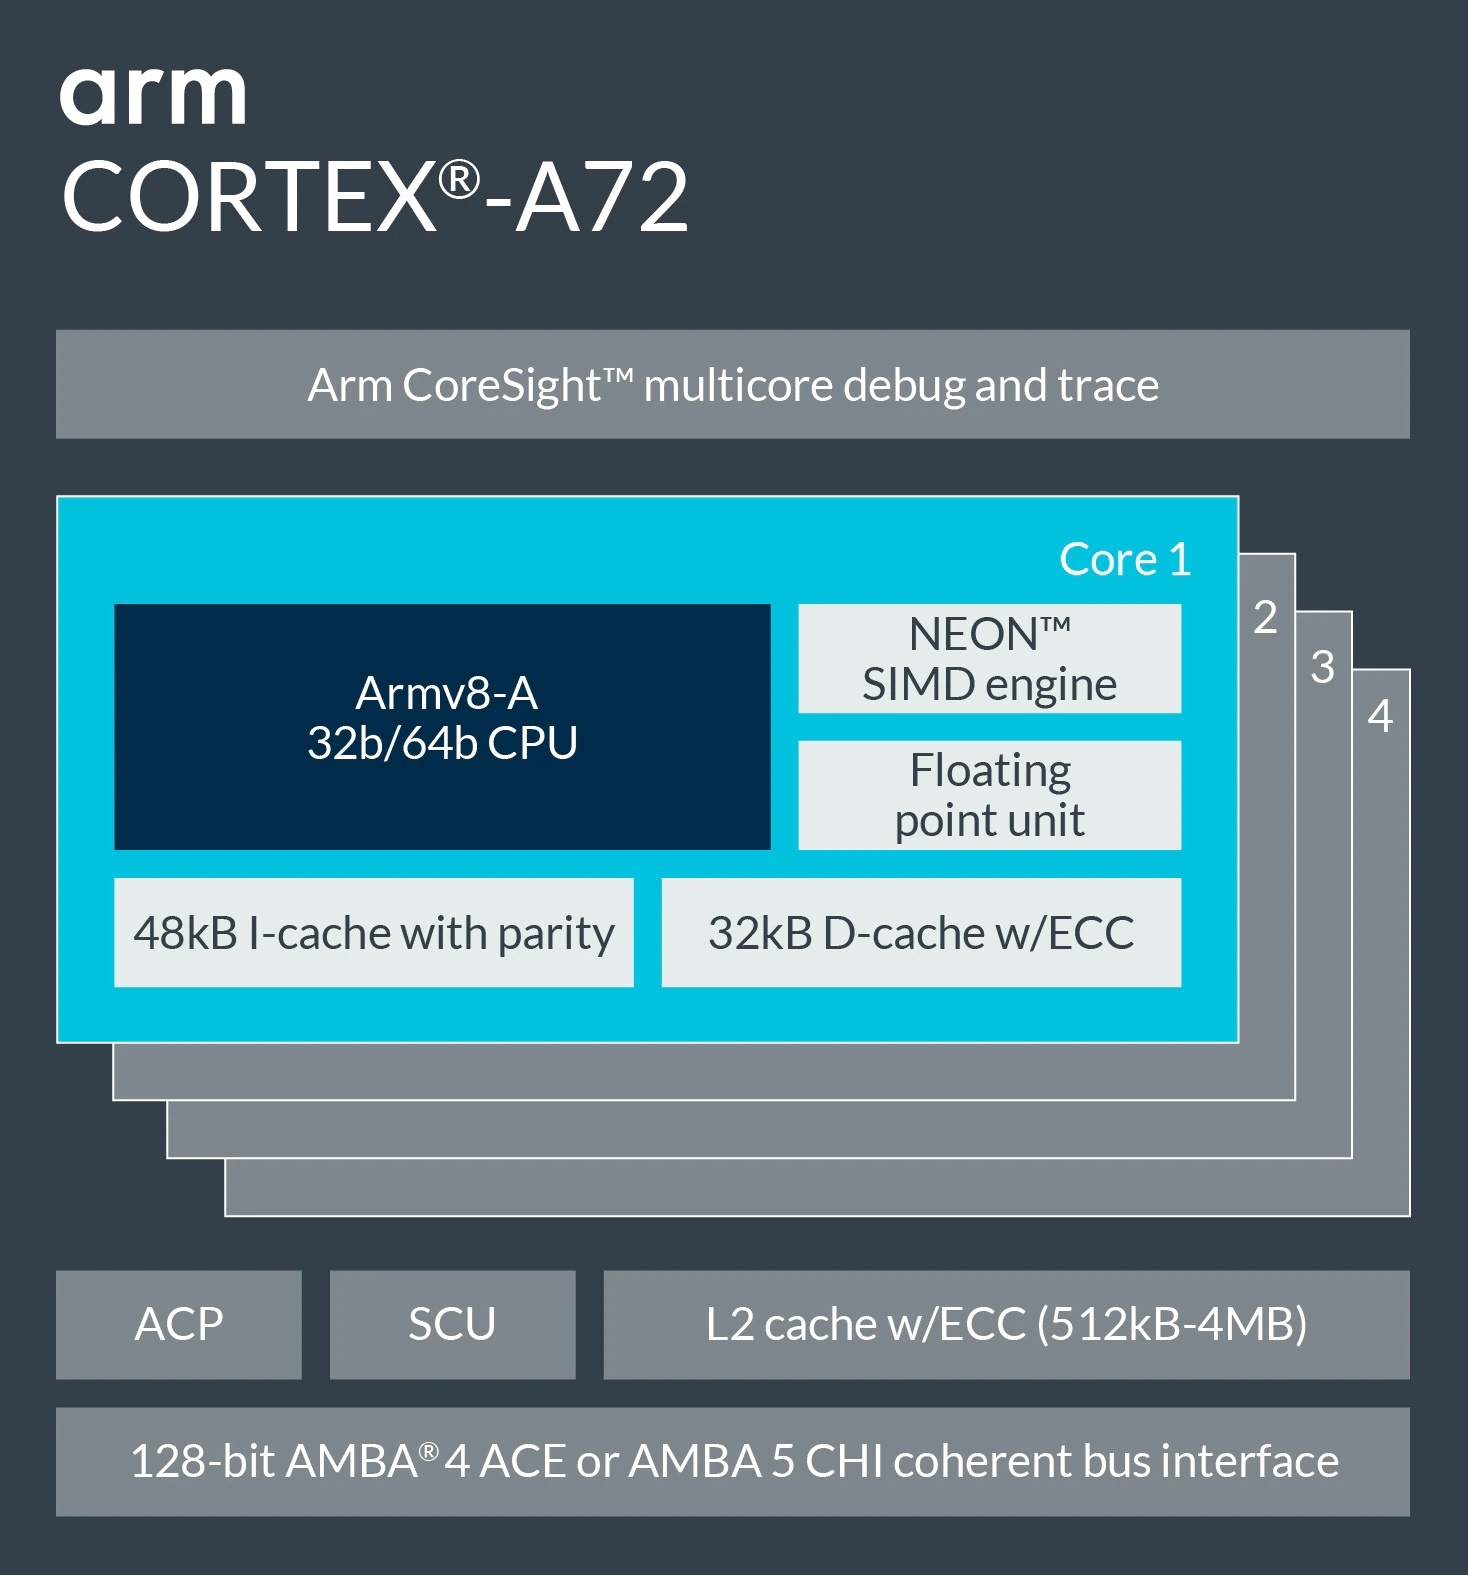
\includegraphics[width=70mm, scale=0.5]{img/Cortex-A72.jpg}
    \caption{Een systematische weergave van de ARM CORTEX-A72 \autocite{armDeveloper2022}}
\end{figure}

\subsubsection{Arduino}
De Arduino is een microcontroller die net zoals de Raspberry Pi \textit{single-board} computer, gebruik maakt van ARM processoren. Het grootste verschil tussen de twee toestellen is dat de Arduino geen mogelijk heeft om videosignalen weer te geven. Dit toestel is in tegenstelling tot de Raspberry Pi uitsluitend gefocust op het automatiseren van processen en het heeft bijgevolg geen besturingssysteem. Deze focus op automatisering leidt ertoe dat het apparaat klein en goedkoop is, zelfs in vergelijking met de Raspberry Pi. Sommige Arduino toestellen zijn reeds verkrijgbaar voor een kostprijs van een tiental euro \autocite{Arduino2018}. 

\subsubsection{Programmable logic controller}
Een \textit{programmable logic controller} (PLC) is een toestel die gebruikt wordt voor het monitoren, loggen en sturen van industriële machines en processen. Deze toestellen zijn de dag van vandaag uiteraard onmisbaar in een wereld waar automatisatie en industrie hand in hand gaan. Eerste generaties van PLC’s werden uitsluitend gebruikt voor het monitoren van sensoren of het aansturen van actuatoren, maar tegenwoordig worden deze toestellen gebruikt voor allerhande toepassingen. Hoewel deze toestellen vroeger vaak gebruik maakten van gepatenteerde besturingssystemen, maken ze de dag van vandaag gebruik van \textit{open source} Linux of Unix besturingssystemen. Deze toestellen zijn tegenwoordig integraal in het concept van \textit{edge computing} die datacenters en gegevensbronnen dichter bij elkaar brengt \autocite{DeCraeke2022}. Een voorbeeld van dit type toestel is de Wago Edge Controller. Dit type PLC maakt gebruik van de ARM Cortex A9 processor \autocite{Wago2022}.

\begin{figure}[!h]
	\centering
	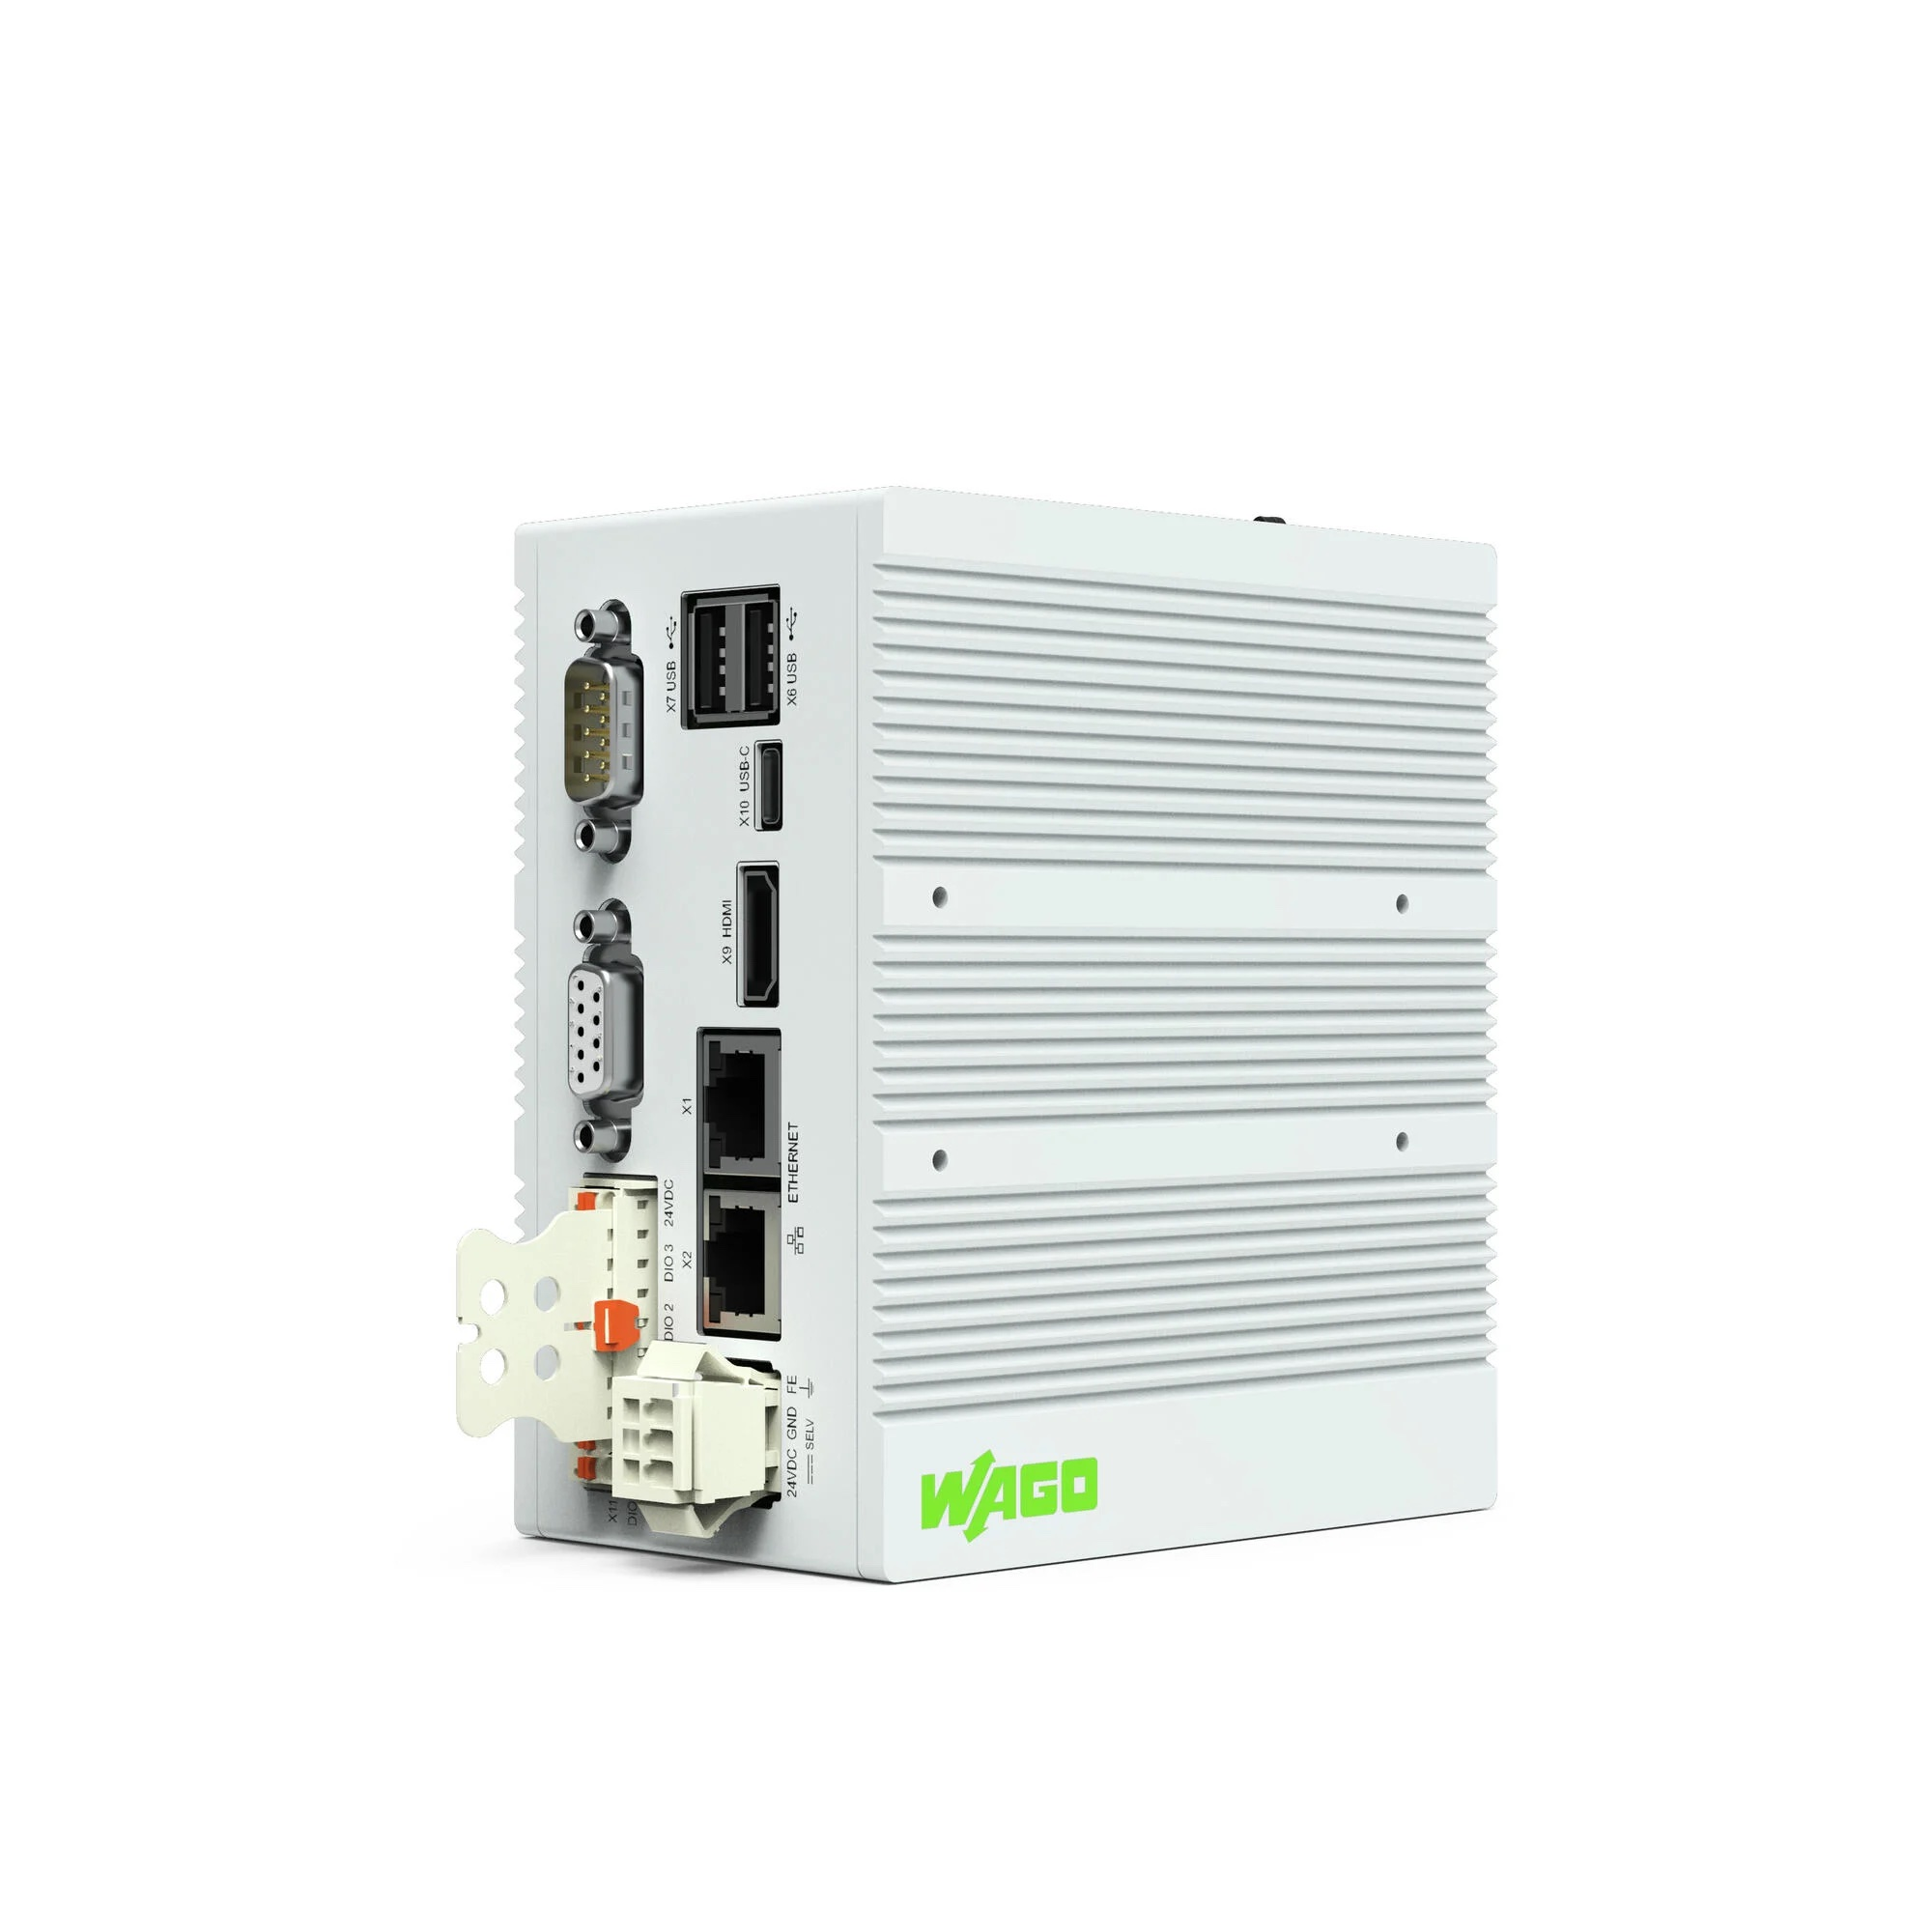
\includegraphics[width=90mm, scale=0.5]{img/wago_edge_controller.jpg}
	\caption{Een Wago PLC Edge Controller \autocite{Wago2022}}
\end{figure}
